% eltonPHYS4699.tex
% $Author: elton $ $Date: 2007-05-02 14:23:51 -0400 (Wed, 02 May 2007) $

        \newif\ifdraft
\drafttrue              % For draft version, commented
%\draftfalse            % For final version, uncomment this

% JRE started LaTeX edits                Jan 18 2007
% PC created project LaTeX template         Jan 13 2007

% http://publish.aps.org/esubs/revtextips.html

 \documentclass[pre,onecolumn,groupedaddress]{revtex4}
% \documentclass[pre,preprint,groupedaddress,showpacs,showkeys]{revtex4}

\input defs         % all definitions in defs.tex
                \begin{document}
                \title{
Another exploration of moderate \Reynolds\ plane Couette turbulence
                }\author{
John R. Elton            }
        \email{
gtg960p@mail.gatech.edu
              }
        \affiliation{
School of Physics\\
Georgia Institute of Technology, Atlanta, GA 30332-0430
                }
               \date{\today}


                \begin{abstract}
The {\tt channelflow} code~\cite{channelflow} for determining
equilibria and unstable periodic orbits of moderate \Reynolds\ plane
Couette turbulence is implemented and applied.

\end{abstract}
\pacs{95.10.Fh, 02.70.Bf, 47.52.+j, 05.45.+a} \keywords{ periodic
orbits, chaos, turbulence, ???
    }
                    \maketitle

\noindent
{\bf Georgia Tech PHYS 4699:}\\
\underline{\bf CHAOS, AND WHAT TO DO ABOUT IT }\\
{\bf special problems project, fall semester 2007}


\section{First Thoughts}
%\label{sec:}
In continuation with the project started in the spring, I would
first like to continue looking into the suspicious region which
traps the trajectories "u1 and u2", see \reffig{u2}. A first list of
various
things to do in order to investigate this region includes: \\
 1.) Run trajectories \emph{starting} in this region. Check out
 any rotational or translational symmetries. \\
 2.) Implement Newton search for equilibria \\
 3.) Search for periodic orbits or relative periodic orbits \\
 4.) Poincare sections \\
 5.) Check out relation and connections to other known equilibria
 regions such as upper or lower branch. \\
 6.) Has anything already been done by JFG or JH? \\

\begin{figure}[!h]
(a)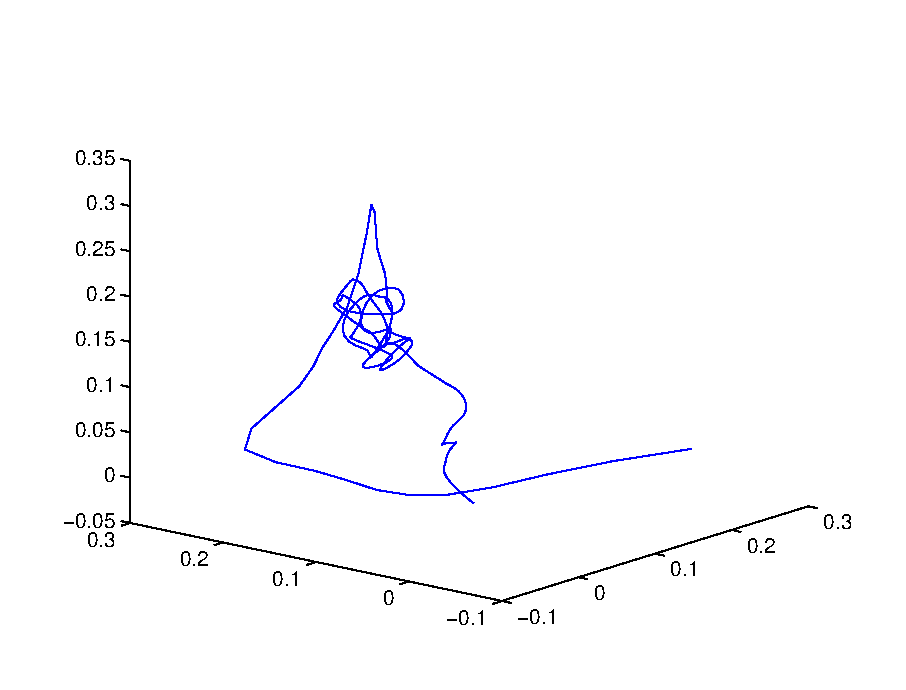
\includegraphics[width=0.40\textwidth]{plot4.eps}
(b)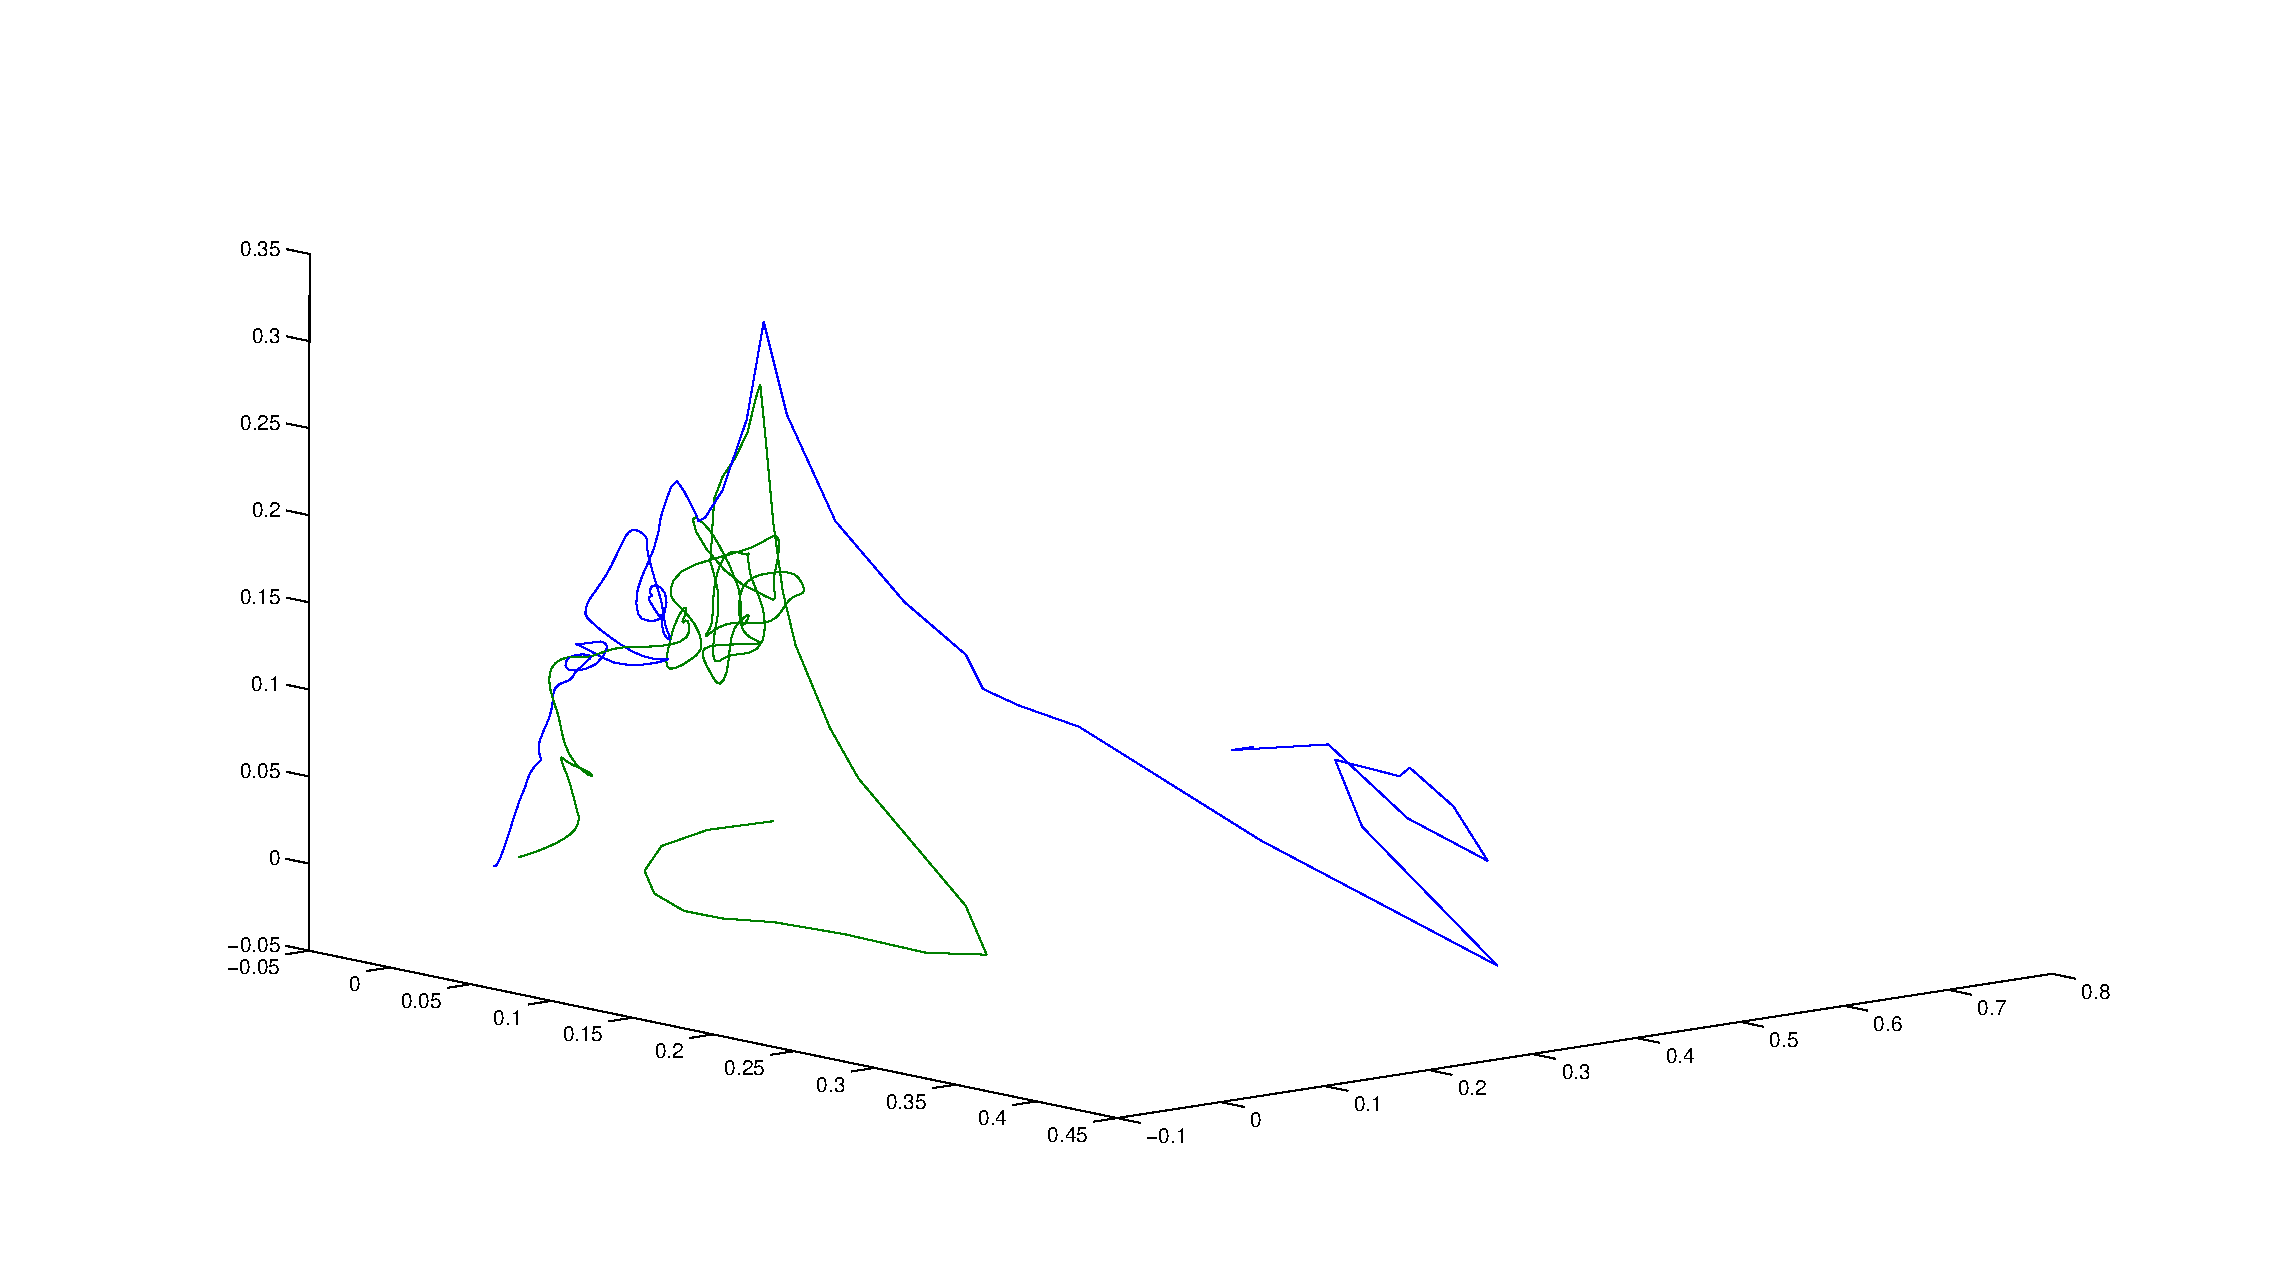
\includegraphics[width=0.50\textwidth]{u1u2.eps}
  \caption{Trajectories
  (a) {u2} (b) {u1 and u2} }
  \label{u2}
 \end{figure}

From the data plotted in \reffig{u2} I narrowed down the range of
 {\tt flowfields} in this region to be approximately between u2(100) and
 u2(200). Picking u2(150) as an initial condition, program {\tt couette}
 produced another trajectory shown in \reffig{u2_1}. Apparently this
 caught the tail end of the knot as it seems to be spiraling away.
 More fishing and thinking to be done.
\begin{figure}[!h]
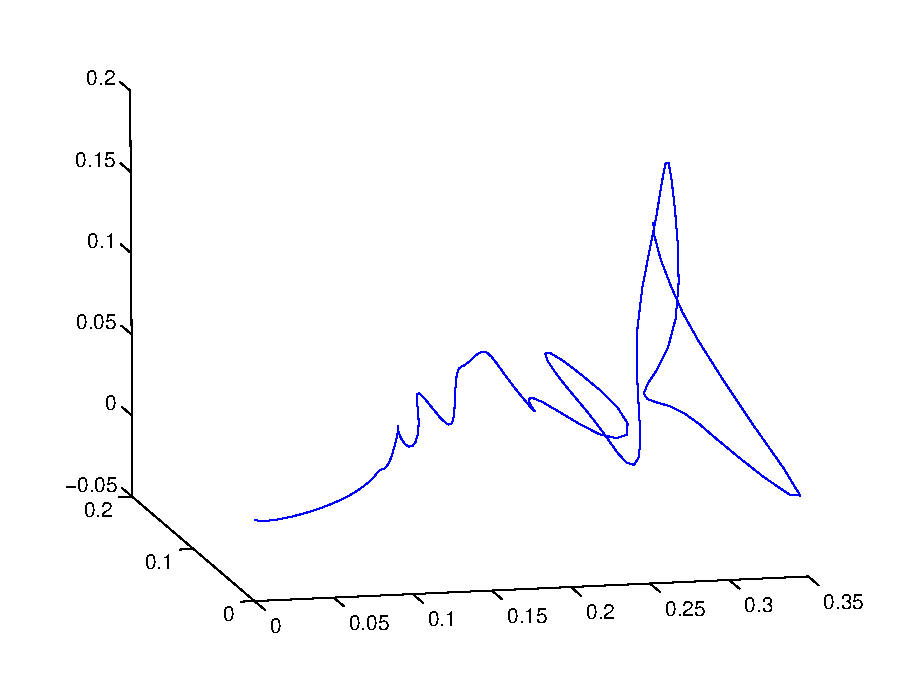
\includegraphics[width=0.40\textwidth]{u2_1.eps}
\caption{u2 new}
  \label{u2_1}
 \end{figure}


 One immediate question that I have which may take some thought or experimentation is about the choice of basis vectors on
 which to project the {\tt flowfields}. The program {\tt makebasis}
 creates an orthonormal basis that is natural for the flow, but the
 user has to implement the \emph{number} of basis vectors on which to
 project. What is a natural choice for this?

 Still trying to catch up on reading blogs and seeing what happened over the
 summer.


%%%%%%%%%%%%%%%%%%%%%%%%%%%%%%%%%%%%%%%%%%%%%%%%%%%%%%%%%%%%%



%%%%%%%%%%%%%%%%%%%%%%%%%%%%%%%%%%%%%%%%%%%%%%%%%%%%%%%%%%%%%

\bibliography{bibtex/elton}

\end{document}
